\subsection{A function built from layers}
A neural network is a parameterized function $f_w$. Given an input $x$, such as an image, it computes an output $\hat y=f_w(x)$. For classification, the output can represent estimated probabilities of several classes. A large output probability expresses the model's confidence; it does not by itself ensure that this confidence is well calibrated or that the prediction is correct.

To begin, suppose an image belongs to exactly one of two classes, cat or dog. A classifier can return two nonnegative numbers summing to one. This differs from a multilabel task, where an image may contain both a cat and a dog: in that case, separate probabilities need not sum to one.

\begin{figure}[htbp]\centering
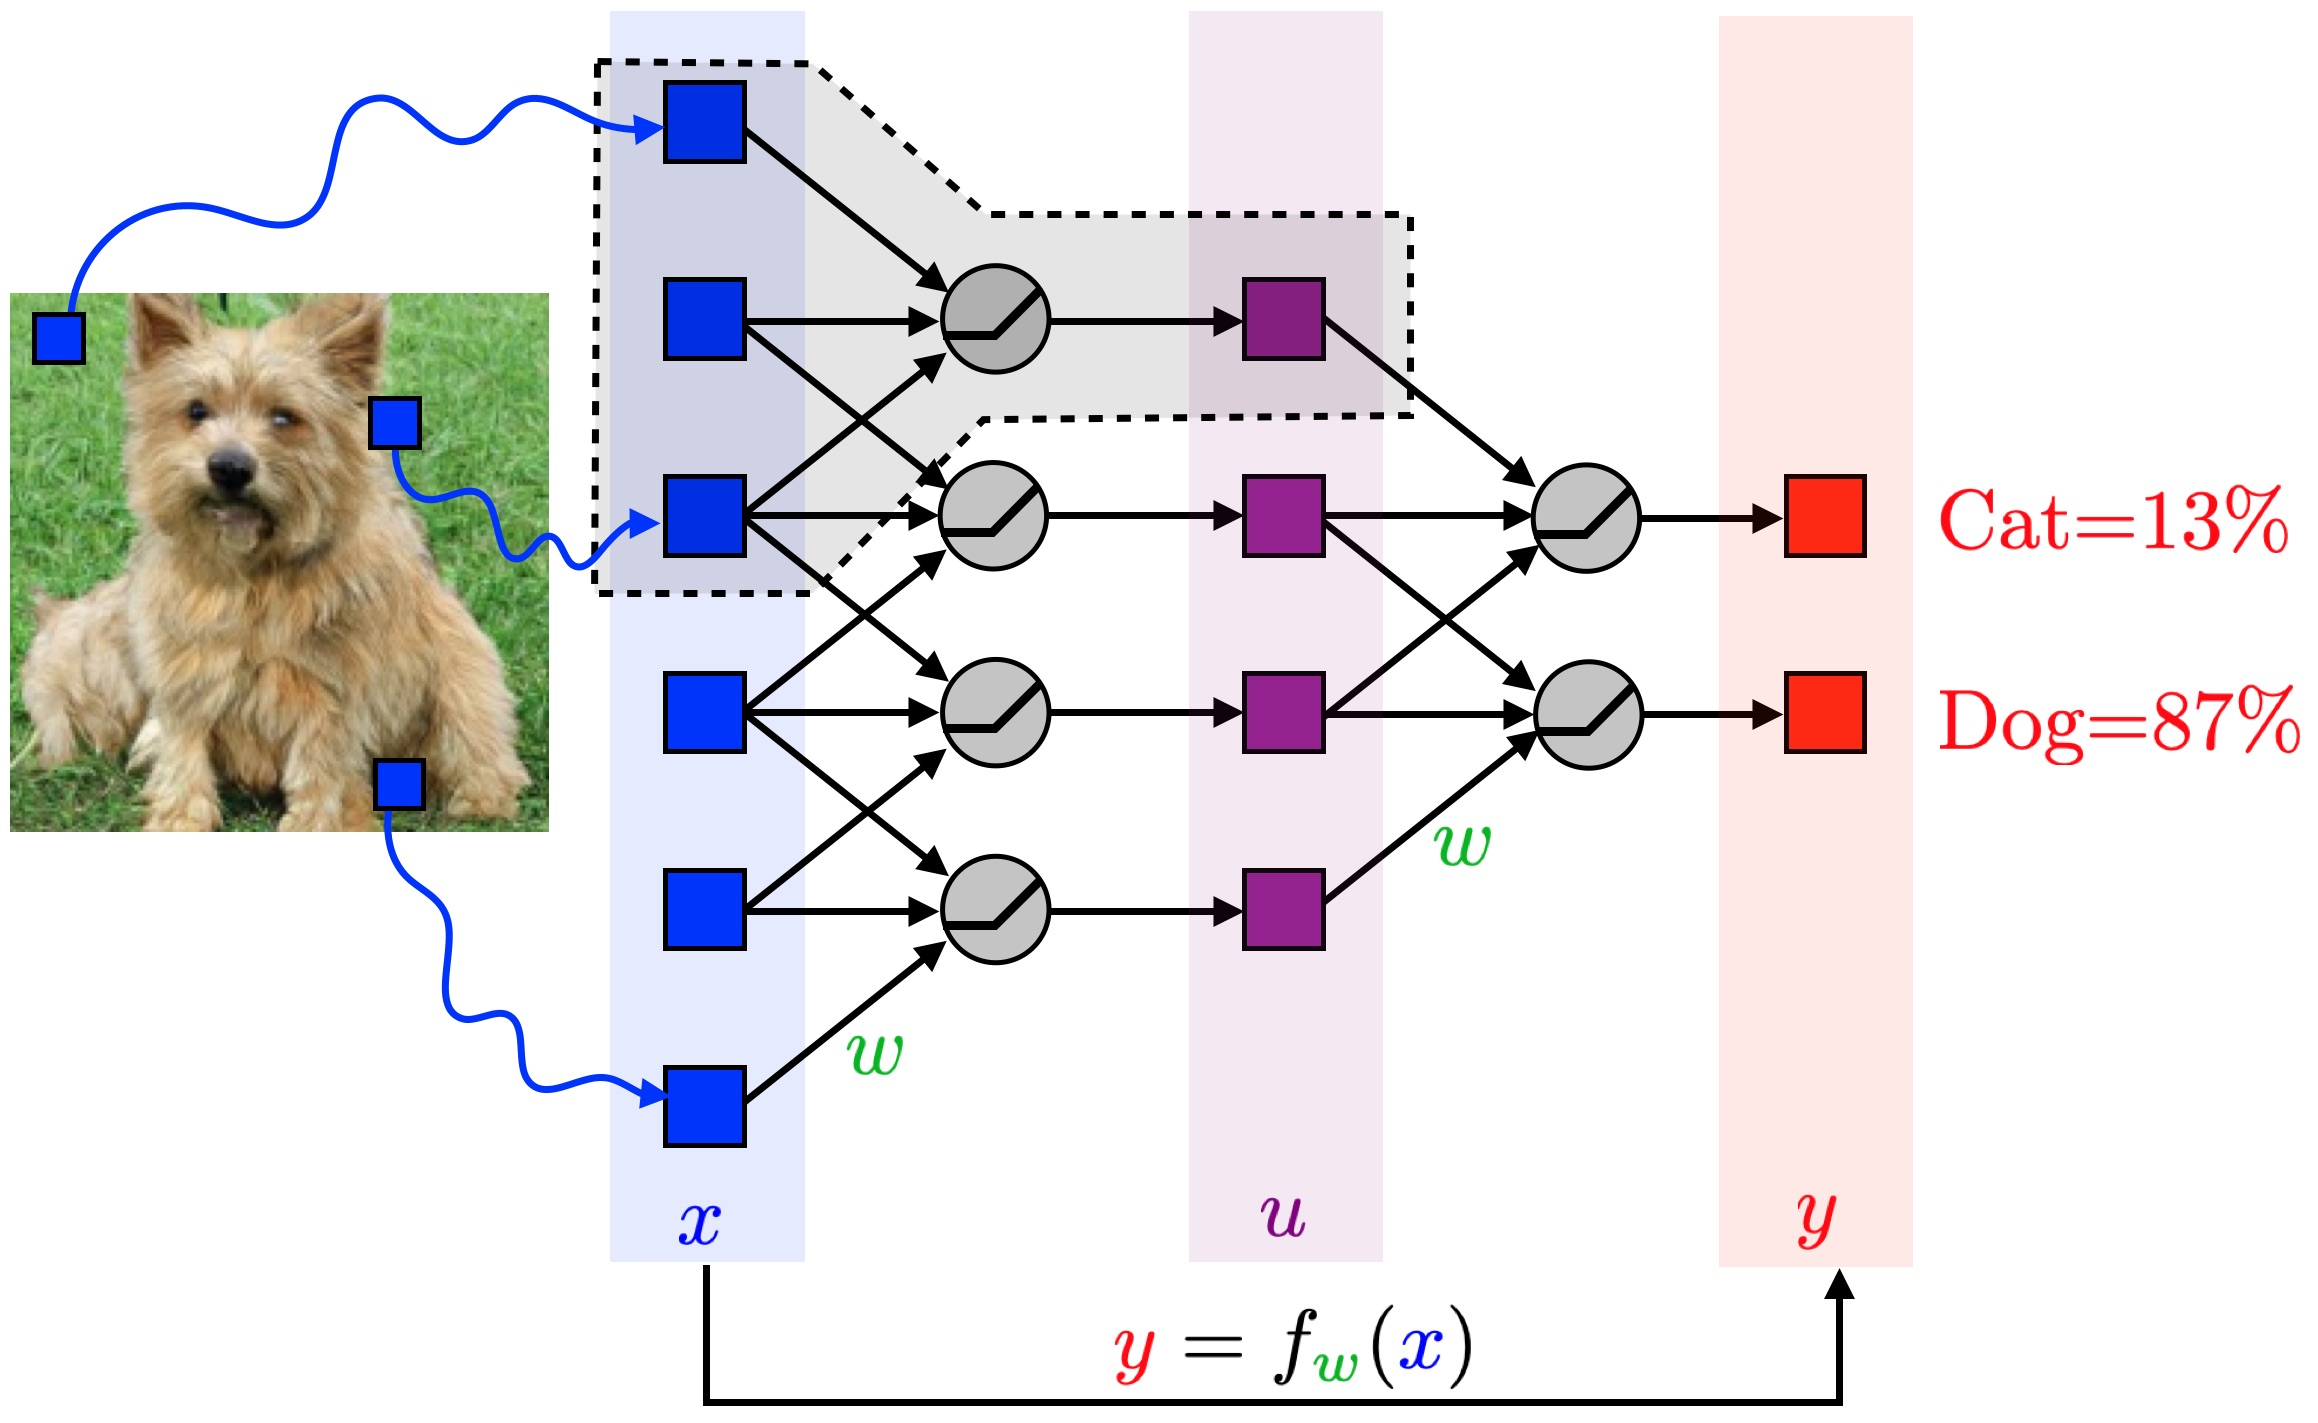
\includegraphics[width=.85\linewidth]{discriminative-en.jpg}
\caption{A schematic classifier with one hidden layer and one output layer. Only a few input pixels and connections are drawn. The displayed percentages are model predictions; a normalization such as softmax is needed to obtain class probabilities.}\label{fig:discriminative}
\end{figure}

Each layer combines affine operations with an activation function. A rectified linear unit, or ReLU, computes
\begin{equation}\label{eq-neuron}
 u_1=\operatorname{ReLU}(w_1x_1+w_2x_2+w_3x_3+b),
 \qquad \operatorname{ReLU}(t)=\max(t,0).
\end{equation}
The weights determine the contribution of each input; the bias $b$ shifts the activation threshold. A ReLU outputs zero for a nonpositive input and passes positive inputs unchanged. It differs from a binary threshold neuron, which has only two possible output values.

\begin{figure}[htbp]\centering
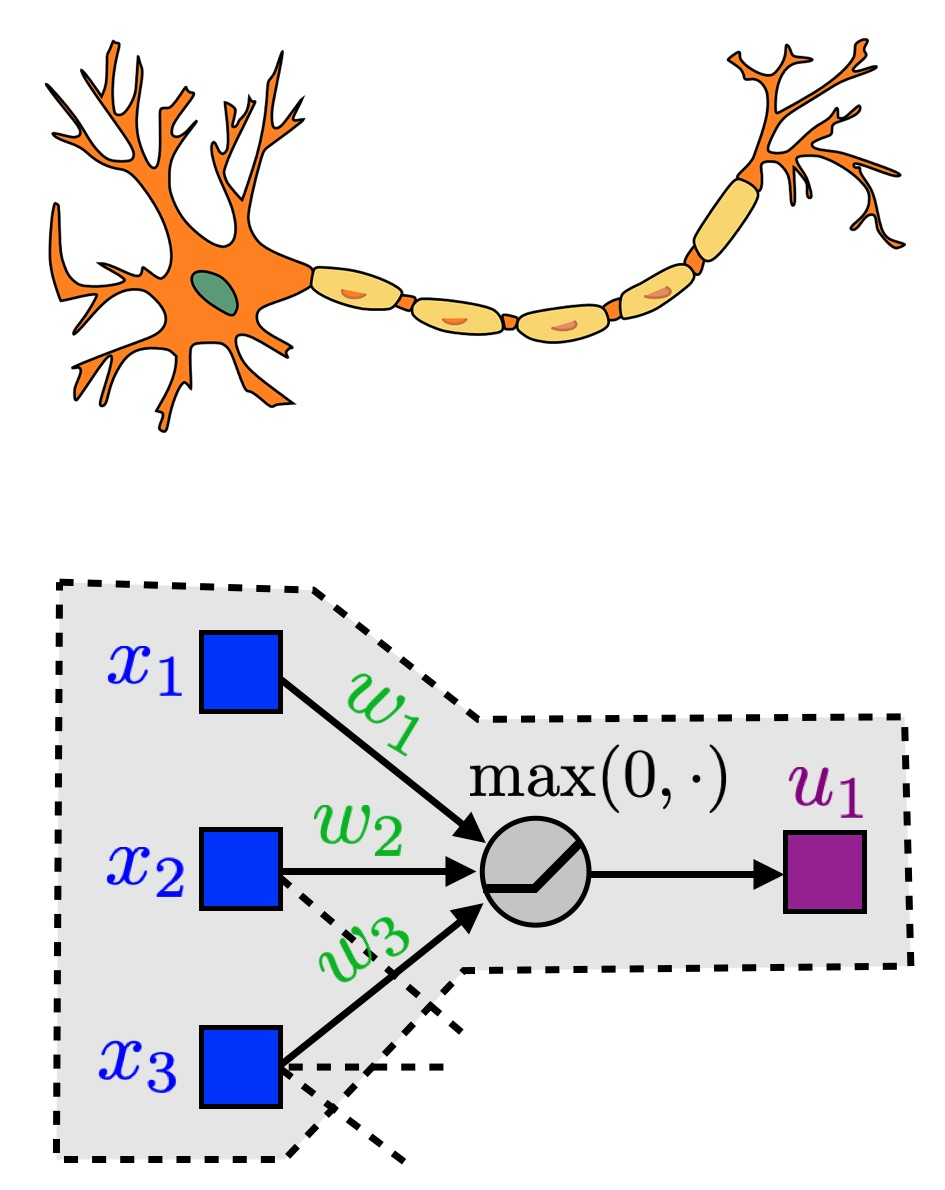
\includegraphics[width=.30\linewidth]{neuron.jpg}
\caption{A biological neuron and a schematic artificial neuron. The mathematical model keeps only a weighted sum and an activation; the bias in~\eqref{eq-neuron} is omitted from the drawing.}\label{fig:neuron}
\end{figure}

For an input $x\in\RR^d$, a hidden layer of width $m$, and $K$ classes, one possible network is
\[
 u=\operatorname{ReLU}(Wx+b),\qquad a=Vu+c,\qquad
 \hat y_k=\frac{e^{a_k}}{\sum_{j=1}^K e^{a_j}},
\]
where $W\in\RR^{m\times d}$, $b\in\RR^m$, $V\in\RR^{K\times m}$, and $c\in\RR^K$. ReLU acts coordinatewise. The final operation is softmax; the intermediate values $a_k$ are called logits. In computation, replacing every $a_k$ by $a_k-\max_j a_j$ gives the same probabilities and avoids overflow. All entries of $W,b,V,c$ form the parameter vector $w$.

Composing more layers gives a deep network. Nonlinear activations are essential: a composition of affine maps is still affine. Depth can represent certain functions more economically than a very wide single hidden layer, but the appropriate architecture depends on the task.

The biological terminology is an analogy, not a faithful model of the brain. McCulloch and Pitts studied logical threshold neurons~\cite{mcculloch1943logical}, while Rosenblatt's perceptron introduced an early learning model~\cite{rosenblatt1957perceptron}. These models should be distinguished from the ReLU networks described here. Biological studies of the visual cortex and of membrane dynamics concern much richer mechanisms~\cite{hubel1962receptive,hodgkin1952quantitative}.

\subsection{Learning from labeled examples}
Supervised learning starts from pairs $(x_i,y_i)_{i=1}^n$. For a single class label $k_i$, the target is often a one-hot vector: $(y_i)_{k_i}=1$, with all other entries zero. Such labels record annotations, rather than known conditional probabilities. The data may come from human annotation or another source of supervision, and may contain mistakes.

\begin{figure}[htbp]\centering
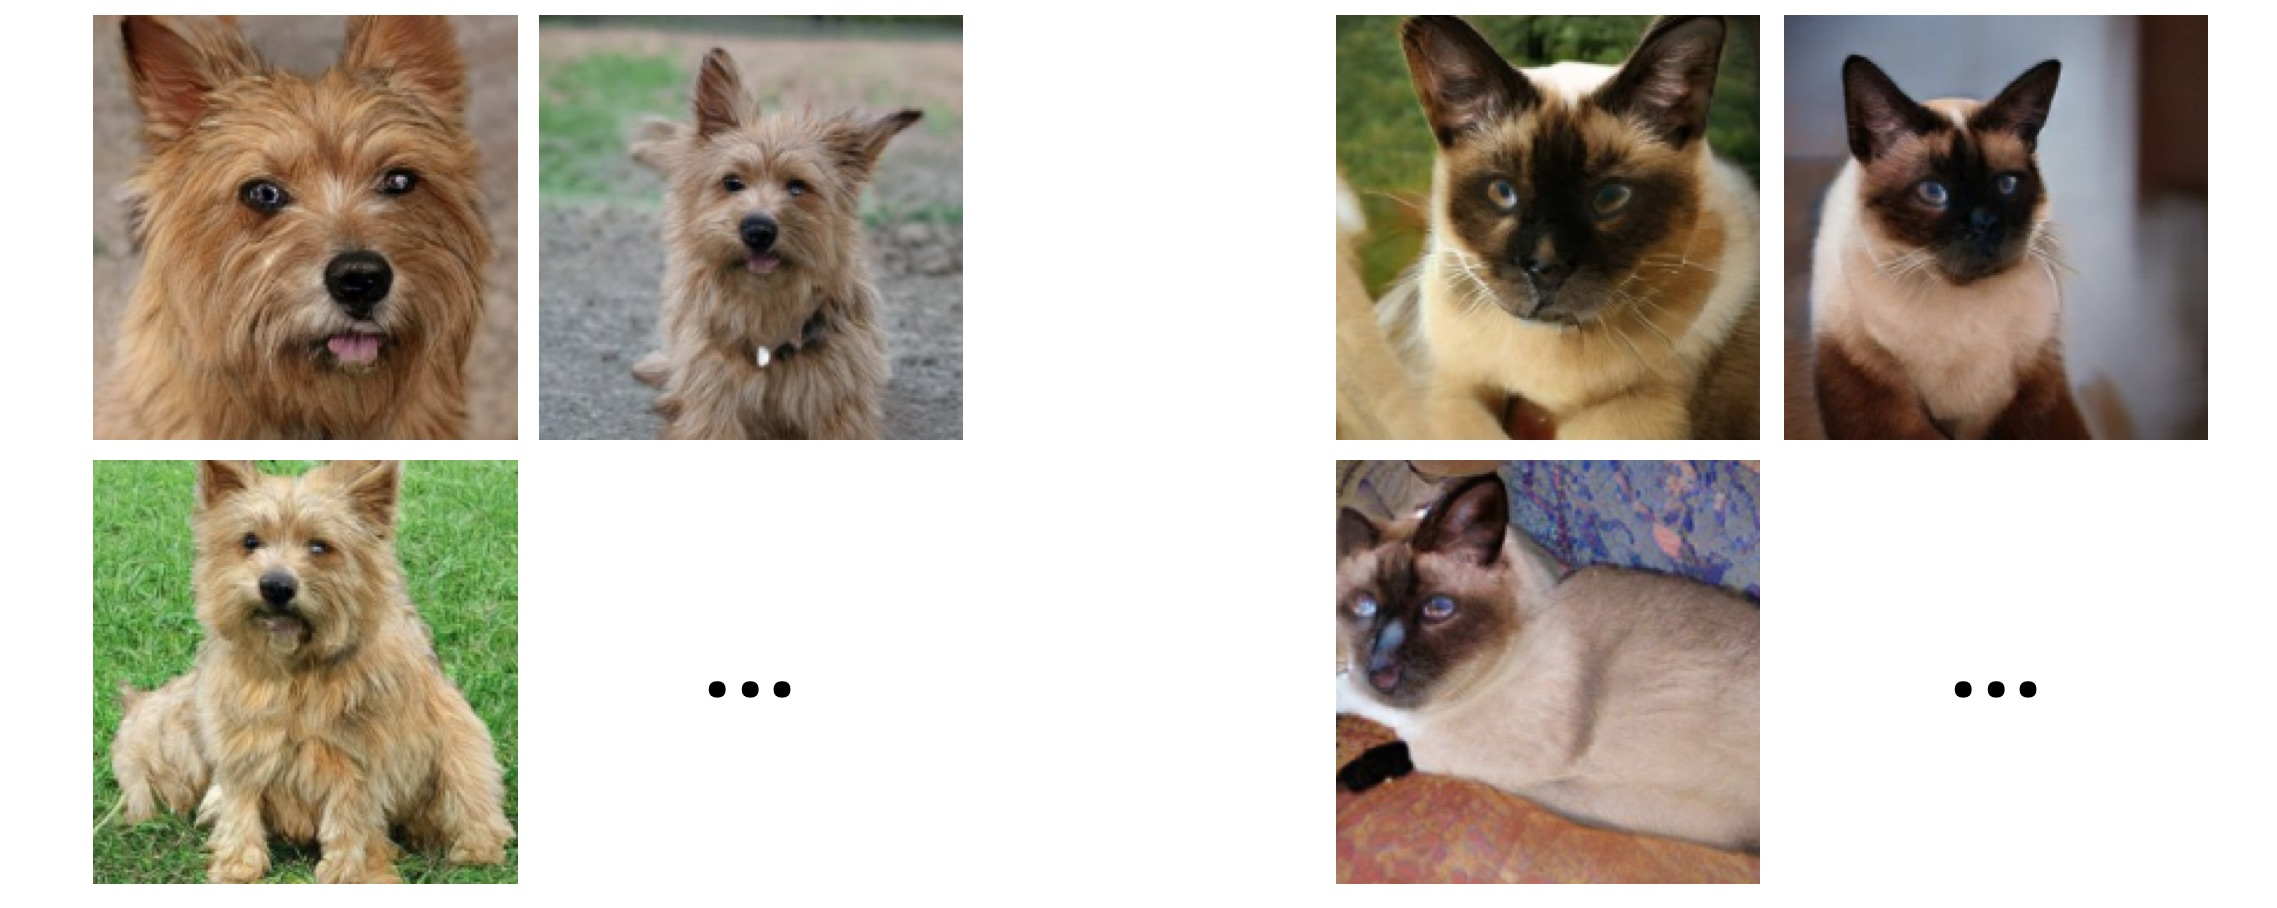
\includegraphics[width=.82\linewidth]{dataset.jpg}
\caption{Examples of labeled dog and cat images from ImageNet~\cite{deng2009imagenet}. Training uses many examples; evaluation requires separate data.}\label{fig:dataset}
\end{figure}

A training objective measures disagreement between predictions and labels. Two examples are the mean squared error and the cross-entropy loss:
\begin{align}
 E_{\mathrm{sq}}(w)&=\frac1n\sum_{i=1}^n\norm{f_w(x_i)-y_i}_2^2,\label{eq-nn-square}\\
 E_{\mathrm{CE}}(w)&=-\frac1n\sum_{i=1}^n\sum_{k=1}^K(y_i)_k\log(f_w(x_i)_k).
 \label{eq-nn-ce}
\end{align}
For a one-hot target, the corresponding cross-entropy term is $-\log(f_w(x_i)_{k_i})$. The logarithm is natural, and softmax gives strictly positive probabilities for finite logits. A stable implementation evaluates the log-softmax directly. A penalty on the weights can be added to the objective.

Training seeks to reduce this empirical loss. Because the network depends nonlinearly on many parameters, the objective is generally nonconvex. Optimization methods can work well without providing a general guarantee of reaching its global minimum.

\subsection{Backpropagation and weight updates}
Backpropagation computes the gradient of a scalar loss by applying the chain rule through the network in reverse order~\cite{rumelhart1986learning,linnainmaa1976taylor}. It is reverse-mode automatic differentiation. An optimizer then uses these derivatives to update the weights; for example, gradient descent takes the step
\[
 w^{(t+1)}=w^{(t)}-\eta_t\nabla E(w^{(t)}),\qquad \eta_t>0.
\]
The step size matters: an excessively large step can increase the loss. Stochastic gradient descent replaces the full gradient by a gradient estimated from a randomly chosen minibatch, reducing the cost of each update. An individual stochastic step need not decrease the full training loss.

For the two-layer classifier above and one example with cross-entropy $\ell$, the chain rule is particularly transparent. Write $r=Wx+b$, $u=\operatorname{ReLU}(r)$, and $\delta=\hat y-y$. Away from $r_j=0$,
\[
 \frac{\partial\ell}{\partial V}=\delta u^\mathsf{T},\qquad
 \frac{\partial\ell}{\partial c}=\delta,\qquad
 q=(V^\mathsf{T}\delta)\odot\mathbf1_{r>0},\qquad
 \frac{\partial\ell}{\partial W}=qx^\mathsf{T},\quad
 \frac{\partial\ell}{\partial b}=q.
\]
Here $\odot$ is coordinatewise multiplication. At a ReLU kink, software chooses a convention, commonly zero, for the derivative of the activation. That convention does not make the network classically differentiable at the kink.

Large labeled datasets, efficient GPU computation, and improvements in architectures and training contributed to the success of deep image classifiers, notably the 2012 ImageNet result~\cite{krizhevsky2012imagenet}. Regularization techniques such as dropout can help limit overfitting~\cite{srivastava2014dropout}. The work of Yoshua Bengio, Geoffrey Hinton, and Yann LeCun was recognized by the 2018 ACM A. M. Turing Award, announced in 2019.\footnote{\url{https://awards.acm.org/about/2018-turing}}

\subsection{Approximation, optimization, and generalization}
A universal approximation theorem concerns what a network can represent. A classical result of Cybenko~\cite{cybenko1989approximation} states that, for a continuous function $F:[0,1]^d\to\RR$ and any $\varepsilon>0$, there exist a finite $m$ and coefficients such that
\[
 G(x)=\sum_{j=1}^m\alpha_j\sigma(v_j\cdot x+\beta_j),
 \qquad \sup_{x\in[0,1]^d}|F(x)-G(x)|<\varepsilon,
\]
where $\sigma$ is a fixed continuous sigmoidal activation, such as $\sigma(t)=1/(1+e^{-t})$. The output layer is linear, and the width and weights are unrestricted. This is the sigmoidal theorem; approximation results for ReLU networks require their own statements.

The theorem does not involve training data. It neither requires infinitely many examples nor guarantees that a training algorithm can find the approximating network from finitely many observations. Three questions must be separated: whether a good representation exists, whether optimization can find it, and whether the learned predictor performs well on new data.

Generalization is evaluated on data excluded from training. Validation data guide choices such as architecture and stopping time; a separate test set estimates the performance of the final procedure. Good performance also depends on whether these data represent the conditions in which the network will be used.

Convolutional networks build in assumptions about spatial structure~\cite{lecun1998gradient}. Local connections restrict the receptive field, and weight sharing applies the same filter at different positions. A stride-one convolution commutes with translations on an infinite or periodic grid; boundary handling and subsampling can change this property. Translation equivariance of a feature map should also be distinguished from translation invariance of a final classification.

Architecture, regularization, data, and optimization all influence performance~\cite{lecun2015deep}. Mathematical results explain particular mechanisms and regimes, while a complete account of every successful architecture remains beyond a single theorem.
